% !TEX root=./report.tex

\subsection{Static Calibration}
\label{sec:static_calibration_approach}

ITS are inherently dependent on the calibration of the different sensors. 
The system has to know the poses of the different sensors relative to some reference coordinate system to accurately measure the position of vehicles within the single sensor ranges and at the overlapping boundaries.

We propose a calibration procedure based on a Bundle Adjustment (BA) problem formulation.
We map visual landmarks in the video feed to their partially known world positions from high definition road maps (HD maps).
We recover the pose by jointly optimizing for the camera intrinsic and extrinsic parameters as well as the real world positions of the landmarks. 

%%%%%%%%%%%%%%%%%%%%%%%%%%%%%%%%%%%%%%%%%%%%%%%%%%%%%%%%%%%%%%%%%%%%%%%%%%%%%%%%%%%%%%%%%%%%%%%%%%%%%%%%%%%%%%%%%%%%%%%%%%%%%%%%%%%%%%%%%%%%%%%%%%%%%%%%%%%%%%%%%
%%%%%%%%%%%%%%%%%%%%%%%%%%%%%%%%%%%%%%%%%%%%%%%%%%%%%%%%%%%%%%%%%%%%%%%%%%%%%%%%%%%%%%%%%%%%%%%%%%%%%%%%%%%%%%%%%%%%%%%%%%%%%%%%%%%%%%%%%%%%%%%%%%%%%%%%%%%%%%%%%
%%%%%%%%%%%%%%%%%%%%%%%%%%%%%%%%%%%%%%%%%%%%%%%%%%%%%%%%%%%%%%%%%%%%%%%%%%%%%%%%%%%%%%%%%%%%%%%%%%%%%%%%%%%%%%%%%%%%%%%%%%%%%%%%%%%%%%%%%%%%%%%%%%%%%%%%%%%%%%%%%

\paragraph{Retrieve Objects from High Definition Maps}

In our project we use HD maps in the \OD{} standard format.
In this work we focus on the permanent delineator (PD) objects that are easily visible in the video feeds.

We extract the world position of the PDs using the mathematical operations defined in the \OD{} standard.
This gives us the the base origin point $o~=~(x, y, z)^T$ of the PDs in the Universal Transverse Mercator (UTM) projection \cite{langley1998utm,proj}. 
This point $o$ is the world position of the lower end of the PD where it touches the ground or another object.
Additionally, we retrieve a directional heading axis $d~=~(x, y, z)^T$ and the height $h$ of the PD.

\paragraph{1D Approximation of Objects}

In the original BA setting the optimization is done jointly over multiple cameras and observations, and the arising stereo vision problem is solved jointly for the 3D positions of the objects and the camera parameters.
For this system of equations to be solvable it requires multiple cameras from different viewing angles and large overlapping fields of view between the cameras.

In our project we have neither of requirements and calibrate each camera separately to the HD map.
We relax the BA problem by the 1D approximation of the PDs
\begin{equation}
S = \{o + \lambda * d: \quad \lambda \in [0, h]\}
\end{equation}
where $S$ is the set of points along its central axis between its base at $\lambda = 0$ and its top at $\lambda = h$.
This approximation allows for a joint optimization of their world positions and the camera intrinsic and extrinsic parameters.

\autoref{sec:static_calibration_number_points} derives a minimal number of points for the resulting system of equations to be solvable.

% The assumptions we made are: 
% \begin{itemize}
  % \item Objects are symmetric around their directional heading axis.
  % \item Projected pixels of the objects are also symmetric around the projected directional axis.
% \end{itemize}


%%%%%%%%%%%%%%%%%%%%%%%%%%%%%%%%%%%%%%%%%%%%%%%%%%%%%%%%%%%%%%%%%%%%%%%%%%%%%%%%%%%%%%%%%%%%%%%%%%%%%%%%%%%%%%%%%%%%%%%%%%%%%%%%%%%%%%%%%%%%%%%%%%%%%%%%%%%%%%%%%
%%%%%%%%%%%%%%%%%%%%%%%%%%%%%%%%%%%%%%%%%%%%%%%%%%%%%%%%%%%%%%%%%%%%%%%%%%%%%%%%%%%%%%%%%%%%%%%%%%%%%%%%%%%%%%%%%%%%%%%%%%%%%%%%%%%%%%%%%%%%%%%%%%%%%%%%%%%%%%%%%
%%%%%%%%%%%%%%%%%%%%%%%%%%%%%%%%%%%%%%%%%%%%%%%%%%%%%%%%%%%%%%%%%%%%%%%%%%%%%%%%%%%%%%%%%%%%%%%%%%%%%%%%%%%%%%%%%%%%%%%%%%%%%%%%%%%%%%%%%%%%%%%%%%%%%%%%%%%%%%%%%

\paragraph{Mapping Objects to Pixels}
\begin{figure}[t]
  \begin{center}
  % \fbox{\rule{0pt}{2in} \rule{0.9\linewidth}{0pt}}
     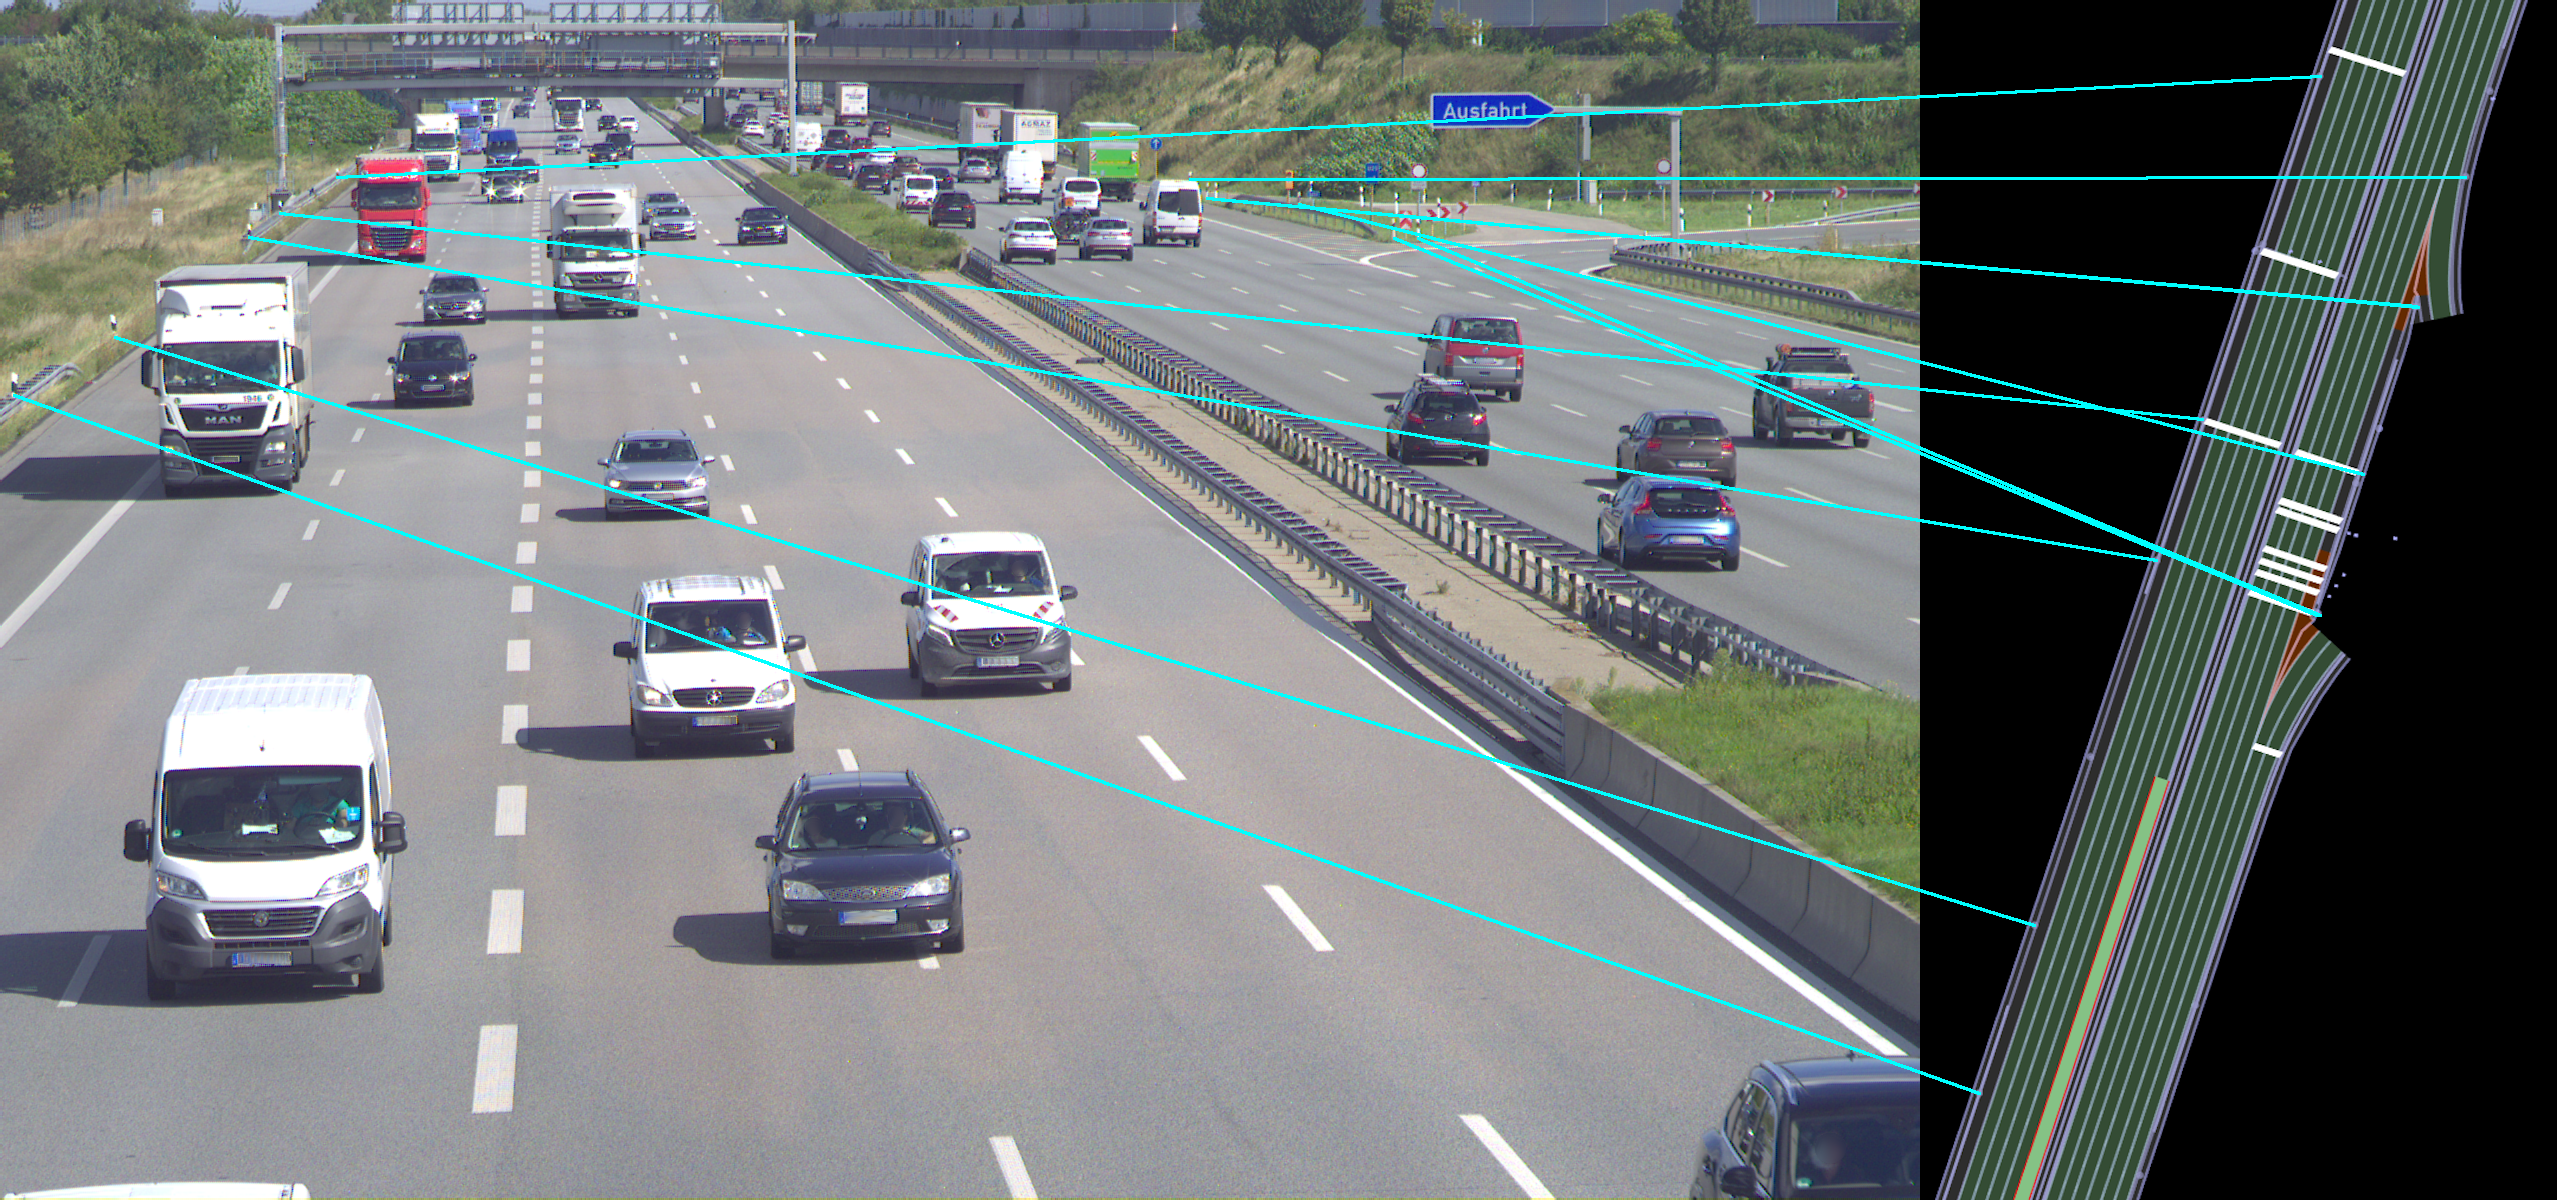
\includegraphics[width=\linewidth]{images/hd_map_mapping.png}
  \end{center}
     \caption{
       Left: The current camera frame. 
       Right: A part of the HD map.
       Light blue lines: An exemplary mapping $s_c \mapsto p_c$ from objects (right) to their corresponding pixels (left).
       }
  \label{fig:static_calibration_mapping}
  \end{figure}

We solve the BA problem by minimizing the reprojection-error over the PDs.
We thus require a set $C$ of correspondences that map world points $s_c$ of the PDs to their respective pixel $p_c$. 

This mapping is currently done by human interaction and not fully automated. 
We implemented an annotation tool to mark pixels that outputs a list of pixels that can easily be mapped to the list of objects.

%%%%%%%%%%%%%%%%%%%%%%%%%%%%%%%%%%%%%%%%%%%%%%%%%%%%%%%%%%%%%%%%%%%%%%%%%%%%%%%%%%%%%%%%%%%%%%%%%%%%%%%%%%%%%%%%%%%%%%%%%%%%%%%%%%%%%%%%%%%%%%%%%%%%%%%%%%%%%%%%%
%%%%%%%%%%%%%%%%%%%%%%%%%%%%%%%%%%%%%%%%%%%%%%%%%%%%%%%%%%%%%%%%%%%%%%%%%%%%%%%%%%%%%%%%%%%%%%%%%%%%%%%%%%%%%%%%%%%%%%%%%%%%%%%%%%%%%%%%%%%%%%%%%%%%%%%%%%%%%%%%%
%%%%%%%%%%%%%%%%%%%%%%%%%%%%%%%%%%%%%%%%%%%%%%%%%%%%%%%%%%%%%%%%%%%%%%%%%%%%%%%%%%%%%%%%%%%%%%%%%%%%%%%%%%%%%%%%%%%%%%%%%%%%%%%%%%%%%%%%%%%%%%%%%%%%%%%%%%%%%%%%%

\paragraph{Calibration procedure}
\begin{figure*}[!ht]
  \centering
  \begin{tabular}{cc}
    \includegraphics[width=0.4\linewidth]{images/calibration/background_uncalibrated_with_mapping.png}    &  
    \includegraphics[width=0.4\linewidth]{images/calibration/background_calibrated.png}    
  \end{tabular}
  \caption{Left: Sampled points of objects that are mapped to pixel locations (green) and sampled points without known corresponding pixels (red) rendered by a poorly calibrated camera model.
  The mapping from the points to their expected pixels is drawn in cyan.
  Right: The same sampled points after the calibration procedure.
  The rendered positions of the sampled points align with the pixels of the objects they are mapped to and the drawn mapping disappears as the distance approaches $0$.  }
  \label{fig:calibration}
  \end{figure*}

Our camera is modelled using the pinhole camera model. 
The pinhole projection from samples of the world objects to pixels is formulated as
\begin{equation}
  \label{eq:static_calibration_reprojection}
  p_c = \pi \left(  
    % \begin{bmatrix}
    %   R, T \\
    %   0, 1
    % \end{bmatrix} *
    R * T *
    (o_c + \lambda_c * h_c)
  \right)
\end{equation}
\begin{equation}
  \label{eq:static_calibration_intrinsic_parameters}
  z * \pi(x) =   
  \begin{bmatrix}
    f_x,& 0,& c_x,& 0\\
    0,& f_y,& c_y,& 0\\
    0,& s,& 1 ,& 0
  \end{bmatrix} * x 
\end{equation}
% \begin{equation}
%   \begin{bmatrix}
%     R, T \\
%     0, 1
%   \end{bmatrix} = 
%   \begin{bmatrix}
%     R, 0 \\
%     0, 1
%   \end{bmatrix} *
%   \begin{bmatrix}
%     0, T \\
%     0, 1
%   \end{bmatrix} =
%   R * T
% \end{equation}

where $R$ is the cameras world rotation in Euler angles, $T$ is the cameras world translation and $\pi$ is the camera projection to image space based on the camera intrinsic parameters.

The optimal value for $\pi,R,T$ is found, if it holds for all correspondences:
\begin{equation}
  0 = p_c - \pi \left( R * T * (o_c + \lambda_c * h_c)\right) = p_c - \hat{p}_c
\end{equation}

This places constraints on the values $\pi,R,T$ can take and enables us to recover the camera pose and intrinsics only from the correspondences.

We estimate the camera pose by minimizing a modified version of the least-squares reprojection error 
\begin{equation}
  \label{eq:static_calibration_error}
  \min_{T, R, \Lambda, W} E(P, S, \pi, T, R, \Lambda, W) 
\end{equation}
formulated as
\begin{equation}
  \begin{split}
  E(P, S, \pi, T, R, \Lambda, W ) =& 
  \sum_{c \in C} 
  \rho(\left\lVert 
    w_c * [ p_c - \hat{p}_c ]
  \right\rVert^2) \\ 
  +& 
  \sum_{c \in C} 
  \alpha * 
  \rho(\left\lVert 
  (1 - w_c)
  \right\rVert^2) \\ 
  +& 
  \sum_{c \in C} 
  \beta * 
  \rho(\left\lVert 
  \Delta(\lambda_c, 0, h_c)
  \right\rVert^2) \\ 
  +& 
  \sum_{\pi_i \in \pi} 
  \gamma *
  \rho(\left\lVert 
  \Delta (\pi_i, \pi_i * 0.9, \pi_i * 1.1)
  \right\rVert^2) \\
  +&
  \delta * 
  \rho(\left\lVert 
  \Delta (R_x, 60, 110)
  \right\rVert^2) \\
  +&
  \delta * 
  \rho(\left\lVert 
  \Delta (R_y, -10, 10)
  \right\rVert^2 
\end{split}
\label{eq:reprojection_error}
\end{equation}
where $P$ is the set of mapped pixels in the image, $S$ is the set of mapped corresponding sampled points from the objects and $\Lambda$ is the set of $\lambda$ values associated with the sampled points.
This formulation allows the optimization over the line approximations of the objects and jointly optimizes for the camera parameters $T, R$ and the $\lambda \in \Lambda$ parameters of the line objects.

The calculation of the exact position of $s_c \sim \lambda$ allows the optimizer to search the whole space of real numbers for $\lambda$.
Nonetheless we penalize values for $\lambda$ that exceed the physical height of the object by 
\begin{equation}
    \Delta (x, l, u) =
    \begin{cases}
      x - u,& \text{if } x > u\\
      x - l,& \text{if } x < l\\
      0,    & \text{else}
    \end{cases} 
\end{equation}
This regularization enables a robust estimation procedure that can flexibly adjust to the missing exact world positions.

\paragraph{Initialization}
In contrast to most pose estimation problems our approach drops the need for good initialization. 
By regularization of the $\lambda$ values enough flexibility is given to optimize over an infinite space of values, 
but enforces the solution of the $\lambda$ to lie within the interval of $\lambda \in [0, h]$.

\begin{equation}
  \bar{s} = \frac{1}{\left\lvert C \right\rvert } \sum_{c \in C} o_c 
\end{equation}

\begin{equation}
  T_0 = \begin{pmatrix}
    1, 0, 0,& \bar{s}_x \\   
    0, 1, 0,& \bar{s}_y \\   
    0, 0, 1,& \bar{s}_z + 1000 \\   
    0, 0, 0,& 1   
  \end{pmatrix}
\end{equation}

\begin{equation}
  R_0 = \mathbb{I} ^ {4 \times 4}
\end{equation}

It is sufficient to initialize with $\lambda_c = 0$ for all correspondences.
The camera rotation is defined to be zero with the camera facing in negative world $z$ axis.
By placing the camera at some distance over the mean of the known object positions with zero rotation the optimization always converges to the desired minimum.

% \begin{itemize}
%   \item HD map based approach
%   \item Optimization algorithm, reprojection error between map and video 
%   \item Landmark extraction, mapping, pose estimation
%   \item Watersheder for pixel marking
%  translation can be  and initializing the camera at the some distance over the mean    
 % \end{itemize}